\UseRawInputEncoding
\documentclass{article}
\usepackage[utf8]{inputenc}
\usepackage[frenchb]{babel}
\usepackage[a4paper]{geometry}
\geometry{margin=2cm}
\usepackage[T1]{fontenc}
\usepackage[hidelinks]{hyperref}
\usepackage{graphicx}
\usepackage{lipsum} 
\usepackage{titlesec}


\usepackage[most]{tcolorbox}
\definecolor{grisClair}{rgb}{0.7529, 0.7529, 0.7529} % RVB (192, 192, 192)

\titleformat*{\section}{\Large\bfseries}
\titleformat*{\subsection}{\large\bfseries} 
\setlength{\parindent}{20pt} 
\setlength{\parskip}{1em} 

\usepackage{xcolor}

\hypersetup{
    colorlinks=true,
    linkcolor=blue,
    urlcolor=blue 
}

\usepackage{listings}

\definecolor{custombrown}{RGB}{150, 75, 0} % Marron moyen clair
\lstset{
    language=Python,
    basicstyle=\ttfamily\small,
    showstringspaces=false,
    breaklines=true,
    keywordstyle=\color{blue},
    commentstyle=\color{custombrown},
    stringstyle=\color{red}
}

\begin{document}

\noindent\hrulefill
\begin{flushright}
    \textbf{\Large SkyCord Documentation}
    
    Samuel DELABRANCHE | Lucas DREANO | Khan-Hasnat UDDIN | Manjot SINGH

    \vspace*{\fill}
    
    \today
\end{flushright}

\newpage
\vspace*{\fill}

\newpage
\noindent\hrulefill
\begin{flushright}
    \large Table des matières 
\end{flushright}
\noindent\hrulefill

\renewcommand{\contentsname}{}
\tableofcontents
\addtocontents{toc}{\protect\setlength{\parskip}{0em}}

\newpage
\phantomsection
\section*{Introduction}
\addcontentsline{toc}{section}{Introduction}

\begin{quote}    
SkyCord représente une plateforme de communication vous offrant une expression personnalisée, une collaboration efficace grâce à des fonctionnalités dédiées aux équipes et une sécurité renforcée pour des échanges privés et protégés. Accessible sur toutes les plateformes, SkyCord garantit une connectivité sans faille sans sacrifier la qualité. Plongez dans cette révolution de la communication en ligne dès à présent !
\vspace*{1\baselineskip}
Ce projet ambitieux est né de la volonté de créer une solution sur mesure répondant aux besoins spécifiques des professionnels des Réseaux et Télécommunications. Conçu comme un logiciel privé, SkyCord s'engage à fournir une plateforme sécurisée où la simplicité d'utilisation se combine à des fonctionnalités avancées, permettant aux professionnels R\&T de gérer efficacement leurs communications et échanges de données confidentielles.

\vspace*{1\baselineskip}
L'objectif majeur derrière la création de SkyCord était de proposer une plateforme flexible et personnalisable, répondant aux exigences de différents secteurs professionnels, tout en assurant la confidentialité absolue des échanges d'informations.

\vspace*{1\baselineskip}
Ainsi, SkyCord se positionne comme un outil indispensable pour les professionnels des Réseaux et Télécommunications, offrant une expérience de communication fluide et sécurisée, spécifiquement conçue pour répondre aux besoins spécifiques des entreprises, tout en garantissant la confidentialité des données échangées.
\end{quote}

\newpage
\phantomsection
\section*{Arborescence}
\addcontentsline{toc}{section}{Arborescence}

\begin{quote}
    
    \begin{center}
        \begin{minipage}{\linewidth}
            Notre application se constitue d'une variété de dossiers et de fichiers qui permettent aux développeurs de bénéficier d'une structure modulaire et organisée. Cette section abordera la structure de notre application en détaillant l'agencement de ses dossiers et fichiers.
    
            Voici alors notre arborescence non détaillée de notre application SkyCord :
    \vspace*{1\baselineskip}
    \begin{center}
                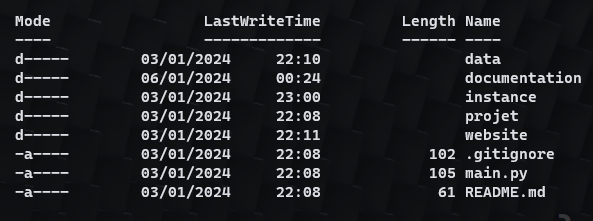
\includegraphics[]{image/arborescence.png}
            \end{center}
    
\vspace*{2\baselineskip}
Tout d'abord, au niveau le plus haut, nous retrouverons les dossiers :
            \begin{center}
                \begin{itemize}
                    \item \textbf{data}
                    \item \textbf{documentation} 
                    \item \textbf{instance} 
                    \item \textbf{projet}
                    \item \textbf{website}
                \end{itemize}
            \end{center}
\vspace*{2\baselineskip}
    Mais aussi nous avons trois fichiers qui sont les suivants :
            \begin{center}
                \begin{itemize}
                    \item \textbf{.gitignore}
                    \item \textbf{main.py}
                    \item \textbf{README.md}
                \end{itemize}
            \end{center}
        \end{minipage}
    \end{center}

    
\end{quote}
\newpage
\begin{quote}
    \addcontentsline{toc}{subsection}{Presentation rapide des différents éléments}

    Voici une brève description des utilités de ces dossiers et fichiers :
    
    \vspace*{1\baselineskip}
    \large{\textbf{data}}

    \begin{quote}
        Contient un fichier "data.json" qui permet de stocker des clés d'authentifications
    \end{quote}

    \vspace*{1\baselineskip}
    \large{\textbf{documentation}}

    \begin{quote}
        Contient tout le nécéssaire permettant de faire ce document
    \end{quote}

    \vspace*{1\baselineskip}
    \large{\textbf{instance}}

    \begin{quote}
        Ce dossier contient le fichier "database.db" qui contient la base de donnée de l'application. \\
        Nous verrons dans la partie "\hyperref[sec:partieFonctions]{Fonctions}" comment est composé ce fichier.
        Cependant, voyez observer l'architecture de celle-ci à l'aide de ce diagramme UML : 
        
        \begin{center}
            \begin{figure}[h]
                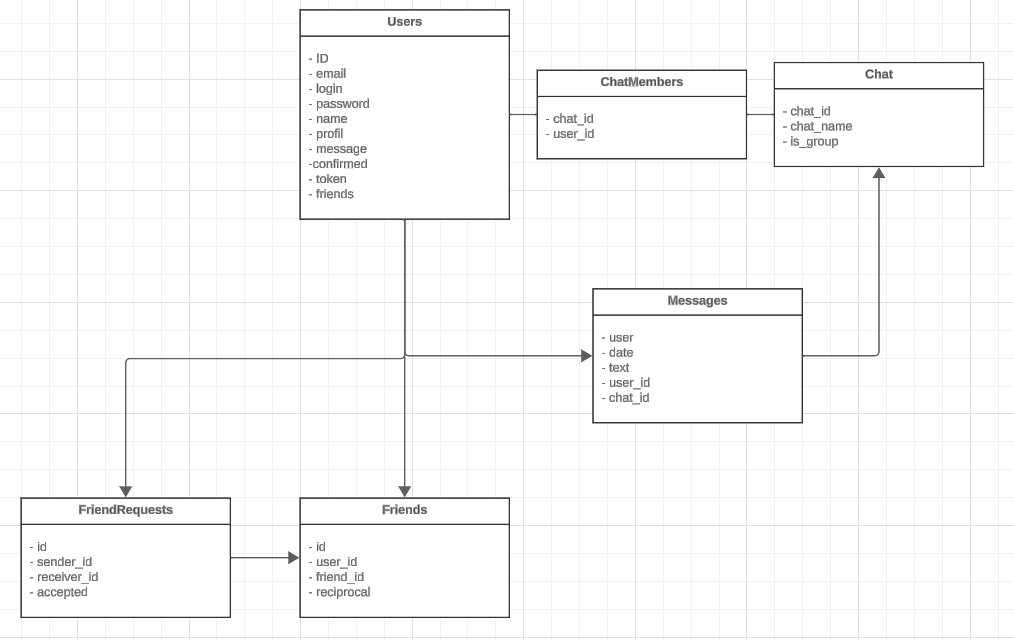
\includegraphics[width=\textwidth]{image/SQL.png}
            \end{figure}
        \end{center}

    \end{quote}

    \newpage

    \large{\textbf{projet}}

    \begin{quote}
        Dossier cœur de notre application. Contient les éléments suivants qui seront présentés dans : \hyperref[sec:partieFonctions]{Fonctions}.
    
        Dossiers :
        \begin{itemize}
            \item \textbf{\_\_pycache\_\_}
            \item \textbf{static} 
            \item \textbf{templates} 
        \end{itemize}
        \vspace*{1\baselineskip}
    
        Fichiers :
        \begin{itemize}
            \item \textbf{\_\_init\_\_.py}
            \item \textbf{auth.py} 
            \item \textbf{friends.py} 
            \item \textbf{models.py} 
            \item \textbf{recup\_info.py} 
            \item \textbf{views.py} 
        \end{itemize}
    \end{quote}
    

    \vspace*{1\baselineskip}
    \large{\textbf{.gitignore}}

    \begin{quote}
        Fichier permettant lors des commits sur notre \href{https://github.com/DreanoLucas/Skycord.git}{GitHub}
        d'éviter d'envoyer certains fichiers et extensions de fichiers.
    \end{quote}
    

    \vspace*{1\baselineskip}
    \large{\textbf{main.py}}

    \begin{quote}
        C'est le fichier coeur de l'application, ce sera le premier qui sera lancé et qui fera lien avec tous les autres pour le bon fonctionnement de notre application.
    \end{quote}

    \large{\textbf{README.md}}
    \vspace*{1\baselineskip}

    \begin{quote}
        Fichier qui permet de décrire le projet sur notre \href{https://github.com/DreanoLucas/Skycord.git}{GitHub}
    \end{quote}

\end{quote}


\newpage
\phantomsection
\section*{Outils utilisés}
\addcontentsline{toc}{section}{Outils utilisés}

\begin{quote}
    Notre équipe à eu besoins d'une multitudes d'outils pour parvenir à la finalité de notre projet. \\

    En voici la liste des plus importants : 

    \begin{itemize}
        \item \textbf{FrameWork Flask :}  
        Flask est un framework web pour Python, léger et simple à utiliser. 
        Il offre des outils pour construire des applications web rapidement et de manière efficace. Sa structure modulaire permet de développer des applications de différentes tailles, de petites API à des applications plus complexes.
        Flask favorise la simplicité et la flexibilité, offrant une grande liberté aux développeurs pour créer des applications web sur mesure. \href{https://flask.palletsprojects.com/en/3.0.x/}{Pour plus d'informations}
        \vspace*{1\baselineskip}
        \item \textbf{SQLite : } 
        SQLite est un système de gestion de base de données relationnelle ultra-léger, parfait pour les petites applications ou projets. 
        Il ne nécessite pas de serveur distinct, stockant toute la base de données dans un simple fichier, simplifiant ainsi son déploiement et sa gestion. \href{https://www.sqlite.org/index.html}{Pour plus d'informations}
        \vspace*{1\baselineskip}
        \item \textbf{GitHub : } 
        GitHub est une plateforme de développement collaboratif basée sur Git, permettant de stocker, gérer et partager efficacement le code source d'un projet. 
        C'est un outil essentiel pour la collaboration, le suivi des modifications et la gestion des versions dans un projet de développement logiciel. \href{https://github.com/}{Pour plus d'informations}
        \vspace*{1\baselineskip}
        \item \textbf{Lucidchart  : } 
        Lucidchart est un outil en ligne de création de diagrammes et de visualisation de données. 
        Il offre des fonctionnalités pour concevoir des organigrammes, des diagrammes de flux, des wireframes et d'autres schémas visuels pour aider à la planification et à la communication dans les projets. \href{https://www.lucidchart.com/pages/fr/exemple/uml-online}{Pour plus d'informations}
        \vspace*{1\baselineskip}
        \item \textbf{Ionicons   : } 
        Ionicons est une bibliothèque d'icônes open source conçue pour être utilisée avec des applications web, mobiles et des interfaces utilisateur. 
        Elle propose une collection d'icônes vectorielles attrayantes et hautement personnalisables pour ajouter des éléments visuels à vos projets. \href{https://ionic.io/ionicons}{Pour plus d'informations}
        \vspace*{1\baselineskip}
        \item \textbf{Replit   : } 
        Replit est une plateforme en ligne qui offre un environnement de développement pour coder, tester et déployer des applications directement depuis le navigateur. Elle supporte plusieurs langages de programmation et fournit des outils pour collaborer avec d'autres personnes sur des projets. 
        De plus, elle permet également l'hébergement de sites web de test pour partager facilement vos créations en ligne. \href{https://replit.com/}{Pour plus d'informations}
    \end{itemize}
\end{quote}

\newpage
\phantomsection
\section*{Fonctions}
\label{sec:partieFonctions}
\addcontentsline{toc}{section}{Fonctions}

\begin{quote}
    Cette section est d'une grande importance, à la fois technique et centrale. Elle explore en détail le fonctionnement de chaque fichier de programmation, principalement en Python, ainsi que leur utilité dans notre processus.

    \textbf{main.py}
    \vspace*{1\baselineskip}
    \begin{quote}
        \begin{tcolorbox}[colback=grisClair,colframe=black]
            \begin{lstlisting}[language=Python]
"""Creates a Flask web application and runs it in debug mode."""
from website import create_app
app = create_app()

if __name__ == '__main__':
    app.run(debug=True)
            \end{lstlisting}
            \end{tcolorbox}
        
        \vspace*{1\baselineskip}
            
    Ce script initialise une application web Flask en appelant create\_app() depuis le module 'website'. Ensuite, il vérifie si le script est exécuté directement et, dans ce cas, démarre l'application Flask en mode débogage. 
    Ce mode débogage permet de déboguer en temps réel et fournit des messages d'erreur détaillés dans le navigateur pendant le développement.
    \end{quote}

    \newpage
    \textbf{\_\_init\_\_.py}
    \vspace*{1\baselineskip}
    \begin{quote}
        \begin{tcolorbox}[colback=grisClair,colframe=black]
        \begin{lstlisting}
"""Configures the Flask application, sets up extensions, defines routes, and initializes the database.

This file sets up the Flask application and its configurations, initializes various extensions
such as SQLAlchemy, Flask-Mail, and Flask-Login. It also defines routes using blueprints for
different parts of the application. Additionally, it includes database initialization logic.

Functions:
    create_app: Initializes and configures the Flask application.
    create_database: Creates the database if it doesn't exist within the 'website' directory.

Dependencies:
    - Flask: Micro web framework for Python.
    - Flask_SQLAlchemy: Flask extension for interacting with SQLAlchemy.
    - Flask-Mail: Flask extension for email functionality.
    - Flask-Login: Flask extension for user session management.

"""

from flask import Flask
from flask_sqlalchemy import SQLAlchemy
from os import path
from flask_mail import Mail, Message
from flask_login import LoginManager
from . import recup_info as rc

db = SQLAlchemy()
DB_NAME = "database.db"
mail = Mail()

def create_app():
    """Creates and configures the Flask application.

    Returns:
        Flask app: The configured Flask application instance.
    """
    app = Flask(__name__)
    code_secret = rc.donnees()
    mail = Mail(app)

    app.config['MAIL_SERVER'] = 'smtp.gmail.com'
    app.config['MAIL_PORT'] = 465
    app.config['MAIL_USE_SSL'] = True
    app.config['MAIL_USERNAME'] = 'skycord.code@gmail.com'
    app.config['MAIL_PASSWORD'] = code_secret['mail_key']
    mail.init_app(app)
    app.config['SECRET_KEY'] = code_secret['flask_key']
    app.config['SQLALCHEMY_DATABASE_URI'] = f'sqlite:///{DB_NAME}'
    db.init_app(app)
    \end{lstlisting}
\end{tcolorbox}  
\begin{tcolorbox}[colback=grisClair,colframe=black]
    \begin{lstlisting}
from .views import views
from .friends import friend
from .auth import auth

app.register_blueprint(views, url_prefix='/')
app.register_blueprint(auth, url_prefix='/')
app.register_blueprint(friend, url_prefix='/')

from .models import User, Message

with app.app_context():
    create_database()

    login_manager = LoginManager() 
    login_manager.login_view = 'auth.login'
    login_manager.init_app(app)

    @login_manager.user_loader
    def load_user(id):
        return User.query.get(int(id))

    return app

def create_database():
"""Creates the database if it doesn't exist.

Checks if the database file exists within the 'website' directory.
"""

if not path.exists('website/' + DB_NAME):
    db.create_all()
    print("Base de donnees creee!")
        \end{lstlisting}
        \end{tcolorbox}
        \vspace*{1\baselineskip}

        Ce fichier est essentiellement un "\textbf{chef d'orchestre}" pour ton site web construit avec Flask. Il rassemble plusieurs tâches importantes :
        \begin{enumerate}
            \item \textbf{Configuration de l'application} : Il met en place l'application Flask et configure différentes parties comme les bases de données, les extensions pour envoyer des emails (\texttt{Flask-Mail}), la gestion des utilisateurs (\texttt{Flask-Login}), etc.
            \item \textbf{Définition des routes} : Il indique comment l'application doit répondre aux demandes des utilisateurs pour différentes parties du site. Par exemple, quand un utilisateur visite la page d'accueil ou essaie de se connecter, ces instructions disent à l'application comment réagir.
            \item \textbf{Initialisation de la base de données} : Il vérifie si la base de données est présente. Si elle n'existe pas, il la crée automatiquement pour stocker des informations comme les utilisateurs, leurs messages, etc.
        \end{enumerate}

        
    \end{quote}
    
    \newpage
    \textbf{auth.py}
    \vspace*{1\baselineskip}
    \begin{quote}
        \begin{tcolorbox}[colback=grisClair,colframe=black]
            \begin{lstlisting}
"""Manages user authentication-related routes and functionalities for the Flask application.

This script contains routes and functions for user authentication purposes within the Flask application.
It includes routes for user login, logout, registration, confirmation email sending, and account confirmation.
Additionally, it defines the authentication blueprint ('auth') and interacts with the database models.

Blueprints:
    auth: Blueprint for handling user authentication-related routes.

Functions:
    login: Handles user login, checking credentials and user confirmation status.
    logout: Handles user logout, terminating the current user session.
    sign_up: Handles user registration, checking input validity and creating new user accounts.
    send_confirmation_email: Sends a confirmation email for account verification.
    confirm_account: Handles user account confirmation using the provided token.

Dependencies:
    - Blueprint: Flask feature for organizing routes.
    - render_template: Function to render HTML templates.
    - request: Object to handle HTTP requests.
    - flash: Function to display flashed messages.
    - redirect: Function to redirect to different routes.
    - url_for: Function to generate URLs for routes.
    - Flask-Mail: Flask extension for email functionality.
    - User: Model for user-related operations from the .models module.
    - db: The database instance.
    - login_user, logout_user, current_user: Functions from Flask-Login for user session management.
    - generate_password_hash, check_password_hash: Functions for password hashing from werkzeug.security.
"""

from flask import Blueprint, render_template, request, flash, redirect, url_for, Flask
from .models import User 
from . import db, mail
import secrets
from flask_login import login_user, login_required, logout_user, current_user
from werkzeug.security import generate_password_hash, check_password_hash
from flask_mail import Mail, Message


auth = Blueprint('auth', __name__)
            \end{lstlisting}       
        \end{tcolorbox}

        \begin{tcolorbox}[colback=grisClair,colframe=black]
        \begin{lstlisting}
@auth.route('/login', methods=['GET', 'POST'])
def login():
    """Handles user login.

    If the request method is POST, it retrieves the username and password from the form.
    It checks if the user exists and, if confirmed, verifies the password.
    Upon successful login, it flashes a success message, logs in the user, and redirects to the home page.

    Returns:
        Flask response or rendered template: Redirects to the home page upon successful login
        or renders the login page.
    """

    if(request.method == 'POST'):
        _username = request.form.get("username")
        _password = request.form.get("password")

        user = User.query.filter_by(login=_username).first()
        if user:
            if user.confirmed == False:
                flash('e-mail non valide', category='error')
            elif check_password_hash(user.password, _password):
                flash('Connecte', category='success')
                login_user(user, remember=True)
                return redirect(url_for('views.home'))
            else:
                flash('Mot de passe incorect', category='error')
        else:
            flash('Aucun compte avec ce nom existe', category='error')

 

    return render_template("page_de_connexion.html")


@auth.route('/logout')
@login_required
def logout():
    """Handles user logout.

    Logs out the current user session using Flask-Login's logout_user() function.
    Upon successful logout, it redirects the user to the login page.

    Returns:
        Flask response: Redirects to the login page after successful logout.
    """
    logout_user()
    return redirect(url_for('auth.login'))

            \end{lstlisting}       
        \end{tcolorbox}
        \begin{tcolorbox}[colback=grisClair,colframe=black]
            \begin{lstlisting}
@auth.route('/sign-up', methods=['GET', 'POST'])
def sign_up():
    """Handles user registration (sign-up).

    If the request method is POST, it retrieves the username, email, and password from the form.
    It checks if the username already exists, validates the email, username, and password length.
    If all conditions are met, it creates a new user in the database, sends a confirmation email,
    and redirects the user to the login page after successful registration.

    Returns:
        Flask response or rendered template: Redirects to the login page upon successful registration
        or renders the sign-up page with error messages.
    """

    if(request.method == 'POST'):
        _username = request.form.get("username")
        _email  = request.form.get("email")
        _password = request.form.get("password")

        user = User.query.filter_by(login=_username).first()
        email = User.query.filter_by(email=_email).first()
        if user:
            flash("Compte deja existant", category='error')
        elif email : flash(f"email deja attribuee au compte {email.login}", category='error')
        elif(len(_email) < 4): flash('Email trop courte', category='error')
        elif(len(_username) < 4): flash('Nom trop court, au moins 4 caracteres est necessaire ', category='error')
        elif(len(_password) < 7): flash('Mot de passe trop court, au moins 7 caracteres est necessaire', category='error')
        
        else : 
            new_user = User(email=_email, login=_username, name=_username, password=generate_password_hash(_password, method='pbkdf2:sha256'), token= secrets.token_urlsafe(30))

            db.session.add(new_user)
            db.session.commit()
            send_confirmation_email(new_user)
            flash('Un email de confirmation a ete envoye a votre adresse.', category='success')
            return redirect(url_for('auth.login'))
    return render_template("page_inscription.html")


          \end{lstlisting}       
        \end{tcolorbox}


    \begin{tcolorbox}[colback=grisClair,colframe=black]
        \begin{lstlisting}
def send_confirmation_email(user):
"""Sends a confirmation email to the user for account verification.

Constructs and sends an email message with a confirmation link to the user's email address.
The link contains a token for account verification, generated using the user's information.

Args:
    user: User object: The user object containing user details (such as email and token).

Returns:
    None
"""

msg = Message('Confirmation de compte', sender='skycord.code@gmail.com', recipients=[user.email])
token = user.token
print(token)
msg.body = f"Pour confirmer votre compte, veuillez cliquer sur le lien suivant: {url_for('auth.confirm_account', token=token, _external=True)}"
print(msg.body)
mail.send(msg)

@auth.route('/confirm_account/<token>')
def confirm_account(token):
    """Handles user account confirmation using the provided token.

    Retrieves a user based on the provided token from the URL parameters.
    If the user exists, it confirms the account by updating the 'confirmed' status and
    removing the token. It logs in the user and displays a success message.
    If the token is invalid or expired, it displays an error message.

    Args:
        token (str): The confirmation token passed in the URL.

    Returns:
        Flask response: Redirects to the home page or renders an error message.
    """
        
    user = User.query.filter_by(token=token).first()

    if user:
        user.confirmed = True
        user.token = None  
        db.session.commit()
        login_user(user, remember=True)
        flash('Votre compte a ete confirme avec succes!', category='success')
    else:
        flash('Le lien de confirmation est invalide ou a expire.', category='error')
    return redirect(url_for('views.home'))


    \end{lstlisting}       
    \end{tcolorbox}
    \newpage
    Ce script Python pour une application Flask gère l'authentification des utilisateurs. Il comprend plusieurs routes et fonctions pour des tâches spécifiques :
    \vspace*{1\baselineskip}
    \begin{enumerate}
    \vspace*{1\baselineskip}
    \item \textbf{Connexion des Utilisateurs :}\\
        La route \texttt{/login} vérifie les identifiants saisis par l'utilisateur. Si les informations sont correctes et que le compte est confirmé, l'utilisateur est connecté.
    \vspace*{1\baselineskip}
        
        \item \textbf{Déconnexion :}\\
        La route \texttt{/logout} permet aux utilisateurs de se déconnecter de leur session en cours.
    \vspace*{1\baselineskip}
        
        \item \textbf{Inscription :}\\
        La route \texttt{/sign-up} gère le processus d'inscription des utilisateurs. Elle vérifie la validité des informations saisies, crée de nouveaux comptes et envoie un e-mail de confirmation.
\\
        \item \textbf{Confirmation de Compte :}\\
        La route \texttt{/confirm\_account/<token>} traite la confirmation du compte à l'aide d'un jeton unique. Si le jeton est valide, le compte est confirmé, l'utilisateur est connecté et un message de succès est affiché.
    \vspace*{1\baselineskip}
        
        \item \textbf{Organisation :}\\
        Le fichier utilise un Blueprint appelé \texttt{auth} pour regrouper les routes liées à l'authentification.
    \vspace*{1\baselineskip}
        
        \item \textbf{Dépendances :}\\
        Il utilise différentes fonctionnalités de Flask telles que \texttt{render\_template}, \texttt{request}, \texttt{flash}, \texttt{redirect}, \texttt{url\_for}, ainsi que l'extension Flask-Mail pour l'envoi d'e-mails.
    \vspace*{1\baselineskip}
        
        \item \textbf{Gestion des Sessions et Sécurité :}\\
        Il utilise Flask-Login pour gérer les sessions utilisateur et \texttt{werkzeug.security} pour le hachage des mots de passe.
    \vspace*{1\baselineskip}
        
        \item \textbf{Fonctions Spécifiques :}\\
        La fonction \texttt{send\_confirmation\_email} envoie un e-mail de confirmation contenant un lien unique pour la vérification du compte utilisateur.
    \end{enumerate}
    \end{quote}

\end{quote}
\newpage
\begin{quote}
    \textbf{friends.py}
    \begin{quote}
        
        \begin{tcolorbox}[colback=grisClair,colframe=black]
            \begin{lstlisting}

"""
Manages friend-related routes and functionalities for the Flask application.

This script contains routes and functions for friend-related functionalities within the Flask application.
It includes routes for adding friends, handling friend requests, displaying friend lists, and managing friend groups.
Additionally, it interacts with the database models for users and friend-related operations.

Blueprints:
    friend: Blueprint for handling friend-related routes.

Functions:
    ajouter: Displays a list of pending friend requests for the current user.
    friend_demand: Displays pending friend requests for the current user.
    groupe: Renders the group page for friends.
    parametre: Renders the settings page for friend-related settings.
    add_friend: Handles the addition of a new friend by sending a friend request.
    accept_demand: Handles the acceptance of a friend request.

Dependencies:
    - Blueprint: Flask feature for organizing routes.
    - render_template: Function to render HTML templates.
    - request: Object to handle HTTP requests.
    - flash: Function to display flashed messages.
    - redirect: Function to redirect to different routes.
    - url_for: Function to generate URLs for routes.
    - Flask-Login: Flask extension for managing user sessions.
    - db: The database instance.
    - FriendRequest, User, Friend: Models for friend-related operations from the .models module.
"""

from flask import Blueprint, render_template, request, flash, redirect, url_for
from . import db
from flask_login import current_user, login_required

from .models import FriendRequest, User, Friend

friend = Blueprint('friend', __name__)
                \end{lstlisting}       
            \end{tcolorbox}

            \begin{tcolorbox}[colback=grisClair,colframe=black]
                \begin{lstlisting}
@friend.route('/ajouter')
@login_required
def ajouter():
    """
    Displays a list of pending friend requests for the current user.

    Returns:
        template: Renders the 'ajouter.html' page with data of pending friend requests.
    """
    amisDemandeListe = []

    friend_requests = FriendRequest.query.filter_by(receiver_id=current_user.id, accepted=False).all()
    for i in friend_requests:
        amisDemandeListe.append(User.query.filter_by(id=i.sender_id).first())
    return render_template('ajouter.html', donnees=amisDemandeListe)

@friend.route('/friend_demand')
@login_required
def friend_demand():
    """
    Displays pending friend requests for the current user.

    Returns:
        template: Renders the 'ajouter.html' page with pending friend requests.
    """
    current_user = User.query.filter_by(login='current_user').first()
    friend_requests = FriendRequest.query.filter_by(receiver_id=current_user.id, accepted=False).all()
    return render_template('ajouter.html', friend_requests=friend_requests)

@friend.route('/groupe')
@login_required
def groupe():
    """
    Renders the group page for friends.

    Returns:
        template: Renders the 'groupe.html' page.
    """
    return render_template('groupe.html')
                    \end{lstlisting}       
                \end{tcolorbox}

    \end{quote}




    \begin{tcolorbox}[colback=grisClair,colframe=black]
        \begin{lstlisting}

@friend.route('/parametre')
@login_required
def parametre():
    """
    Renders the settings page for friend-related settings.

    Returns:
        template: Renders the 'page_parametre.html' page.
    """
    return render_template('page_parametre.html')

@friend.route('/add_friend', methods=['POST'])
@login_required
def add_friend():
    """
    Handles adding a new friend by sending a friend request.

    Returns:
        redirection: Redirects to the home page ('views.home') after processing the request.
    """
    if request.method == 'POST':
        friend_name = request.form['friend_name']

        ami_exist = User.query.filter_by(login=friend_name).first()
        if ami_exist:
            existing_request = FriendRequest.query.filter_by(sender_id=1, receiver_id=ami_exist.id, accepted=False).first()

            if existing_request:
                flash(f"A friend request is already pending for {friend_name}.", category='error')
            else:
                current_user = User.query.filter_by(login='current_user').first()
                new_request = FriendRequest(sender_id=current_user.id, receiver_id=ami_exist.id)
                db.session.add(new_request)
                db.session.commit()
                flash(f"Friend request sent to {friend_name}. Please wait for confirmation.", category='success')

        else:
            flash(f"{friend_name} does not exist.", category='error')

    return redirect(url_for('views.home'))

            \end{lstlisting}       
        \end{tcolorbox}

        \begin{tcolorbox}[colback=grisClair,colframe=black]
            \begin{lstlisting}

@friend.route('/accept_demand/<int:demande_id>', methods=['POST'])
def accept_demand(demande_id):
    """
    Handles the acceptance of a friend request.

    Args:
        demande_id (int): The ID of the friend request to accept.

    Returns:
        redirection: Redirects to the friend_demand route after processing the request.
    """
    friend_request = FriendRequest.query.get(demande_id)

    if friend_request:
        friend_request.accepted = True

        friend_entry_1 = Friend(user_id=friend_request.sender_id, friend_id=friend_request.receiver_id)
        friend_entry_2 = Friend(user_id=friend_request.receiver_id, friend_id=friend_request.sender_id, reciprocal=True)

        db.session.add_all([friend_entry_1, friend_entry_2])
        db.session.commit()

        flash(f"You are now friends with {friend_request.sender.name}.", category='success')
    else:
        flash("Friend request not found.", category='error')

    return redirect(url_for('friend.friend_demand'))


                \end{lstlisting}       
            \end{tcolorbox}
            \vspace*{1\baselineskip}
\textbf{Ce fichier Python} pour une application \textbf{Flask} \textbf{gère} les fonctionnalités liées aux \textbf{amis}. 
Il permet aux utilisateurs d'\textbf{ajouter} des \textbf{amis}, de \textbf{gérer} les \textbf{demandes d'amis} en attente, 
d'\textbf{afficher} les listes d'\textbf{amis} et de \textbf{configurer} des \textbf{paramètres} relatifs aux \textbf{amis}, comme les pages de \textbf{groupe}. 
C'est essentiellement un ensemble d'\textbf{outils} qui permet aux utilisateurs de \textbf{gérer} leurs \textbf{relations} avec d'autres utilisateurs de l'application.
\end{quote}

\newpage
\textbf{models.py}
\vspace*{1\baselineskip}
\begin{quote}


\begin{tcolorbox}[colback=grisClair,colframe=black]
    \begin{lstlisting}
"""Handles the database models for user authentication and message storage.

This script defines two SQLAlchemy models: 'User' and 'Message'. 
- 'User' represents user details and authentication information.
- 'Message' stores messages associated with users.

Classes:
    Message: Represents stored messages, linked to User.
    User: Represents user details and authentication.

Dependencies:
    - db: The database instance.
    - UserMixin: Flask-Login helper class for User model.

Note:
    Ensure the models align with your application's authentication and message storage requirements.
"""

from . import db
from flask_login import UserMixin
from sqlalchemy.sql import func

class User(db.Model, UserMixin):
    id = db.Column(db.Integer, primary_key=True)
    email = db.Column(db.String(50), unique=True, nullable=False)
    login = db.Column(db.String(30), unique=True, nullable=False)
    password = db.Column(db.String(20), nullable=False)
    name = db.Column(db.String(20), nullable=False)
    profil = db.Column(db.String(250)) 
    message = db.relationship('Message')
    confirmed = db.Column(db.Boolean, default=False)
    token = db.Column(db.String(100))
    friends = db.relationship('Friend', foreign_keys='Friend.user_id', backref='user', lazy=True)

class Chat(db.Model):
    chat_id = db.Column(db.Integer, primary_key=True)
    chat_name = db.Column(db.String(100))
    is_group = db.Column(db.Boolean, default=False) # a voir si c'est utile

    \end{lstlisting}       
\end{tcolorbox}


\begin{tcolorbox}[colback=grisClair,colframe=black]
    \begin{lstlisting}
        class ChatMember(db.Model):
        chat_id = db.Column(db.Integer, db.ForeignKey('chat.chat_id'), primary_key=True)
        user_id = db.Column(db.Integer, db.ForeignKey('user.id'), primary_key=True)
      
      class Message(db.Model):
        id = db.Column(db.Integer, primary_key=True)
        date = db.Column(db.DateTime(timezone=True), default=func.now())
        text = db.Column(db.String(1000), nullable=False)
        user_id = db.Column(db.Integer, db.ForeignKey('user.id'))
        chat_id = db.Column(db.Integer, db.ForeignKey('chat.chat_id'))
      
      class Friend(db.Model):
          id = db.Column(db.Integer, primary_key=True)
          user_id = db.Column(db.Integer, db.ForeignKey('user.id'), nullable=False)
          friend_id = db.Column(db.Integer, db.ForeignKey('user.id'), nullable=False)
          reciprocal = db.Column(db.Boolean, default=False)
          
      class FriendRequest(db.Model):
          id = db.Column(db.Integer, primary_key=True)
          sender_id = db.Column(db.Integer, db.ForeignKey('user.id'), nullable=False)
          receiver_id = db.Column(db.Integer, db.ForeignKey('user.id'), nullable=False)
          accepted = db.Column(db.Boolean, default=False)
    \end{lstlisting}       
\end{tcolorbox}

\vspace*{1\baselineskip}
    
Ce script Python gère les modèles de base de données essentiels pour l'authentification des utilisateurs et le stockage des messages dans une application développée avec Flask, un framework web. 
Il introduit différents modèles SQLAlchemy qui structurent la base de données pour gérer les détails des utilisateurs, les fonctionnalités de messagerie, les amitiés et les demandes d'amis. Voyons en détail :

\begin{enumerate}
    \vspace*{1\baselineskip}
    \item \textbf{User} : Définit la structure de l'entité 'Utilisateur', regroupant les données relatives à l'utilisateur telles que l'e-mail, les identifiants de connexion, les informations de profil et les détails d'authentification. Il gère également les relations avec les messages, les amis et les demandes d'amis.
    \vspace*{1\baselineskip}
    \item \textbf{Message} : Représente les messages associés aux utilisateurs. Il lie les messages aux utilisateurs et fournit des détails tels que le contenu du message, l'horodatage et le chat associé.
    \vspace*{1\baselineskip}
    \item \textbf{Chat} : Décrit la structure d'un chat, détaillant des propriétés telles que l'identifiant du chat, le nom et s'il s'agit d'un chat de groupe ou non.
    \vspace*{1\baselineskip}
    \item \textbf{ChatMember} : Gère la relation entre les utilisateurs et les chats, associant les utilisateurs à des chats spécifiques.
    \vspace*{1\baselineskip}
    \item \textbf{Friend \& FriendRequest} : Gèrent les fonctionnalités liées à l'amitié en définissant la structure des amis et des demandes d'amis. Le modèle 'Friend' maintient des informations sur les amitiés, tandis que le modèle 'FriendRequest' gère les demandes d'amis en attente entre utilisateurs.
\end{enumerate}
Les modèles sont interconnectés à l'aide de différentes clés étrangères et relations pour établir un schéma de base de données structuré et interconnecté qui permet l'authentification, la messagerie et les fonctionnalités liées aux amis dans l'application Flask.

\end{quote}

\newpage
\textbf{recup\_info.py}
\vspace*{1\baselineskip}
\begin{quote}
    
\begin{tcolorbox}[colback=grisClair,colframe=black]
    \begin{lstlisting}
"""Handles loading data from a JSON file.

This script contains a function 'donnees' to read data from a specified JSON file path
and return it as a Python dictionary. It manages file-related exceptions such as file not
found or JSON decoding errors, displaying error messages when necessary.

Functions:
    donnees: Loads data from a JSON file and returns its content as a dictionary.

Dependencies:
    json: Module for JSON data encoding and decoding.
"""

import json

def donnees(nom_fichier = "data/data.json"):
    """Loads data from a JSON file.

    Attempts to open and read the specified JSON file and returns its contents as a Python dictionary.

    Args:
        nom_fichier (str, optional): The path to the JSON file. Defaults to "data/data.json".

    Returns:
        dict or None: A dictionary containing the data from the JSON file, or None if an error occurs.
    
    Raises:
        FileNotFoundError: If the specified file is not found.
        json.JSONDecodeError: If there's an error decoding the JSON data.
    """
    try:
        with open(nom_fichier, 'r') as fichier :
            donnees = json.load(fichier)
            return donnees
    except FileNotFoundError:
        print(f"Le fichier {nom_fichier} n'a pas ete trouve.")
        return None
    except json.JSONDecodeError as e:
        print(f"Erreur de decodage JSON : {e}")
        return None

if __name__ =="__main__" :
    print(donnees())
    \end{lstlisting}       
\end{tcolorbox}

\vspace*{1\baselineskip}
Ce script Python charge des données à partir d'un fichier JSON. Il propose une fonction appelée donnees qui lit le contenu d'un fichier JSON spécifié et le renvoie sous forme d'un dictionnaire Python. En cas de problème, comme un fichier introuvable ou une erreur de décodage JSON, il affiche un message d'erreur. 

\end{quote}

\newpage
\textbf{views.py}
\vspace*{1\baselineskip}
\begin{quote}
    
\begin{tcolorbox}[colback=grisClair,colframe=black]
    \begin{lstlisting}
"""Defines routes and views for the application.

This script contains routes and views using Flask's Blueprint functionality.
It includes a route for the home page ('/') that renders the 'acceuil.html' template.
Blueprints:
    views: Blueprint for handling application views and routes.
Functions:
    home: Renders the home page, ensuring the user is logged in using Flask-Login's login_required.
Dependencies:
    - Flask: Micro web framework for Python.
    - Blueprint: Flask feature for organizing routes.
    - render_template: Function to render HTML templates.
    - login_required: Decorator from Flask-Login for requiring login to access routes.
    - current_user: Function from Flask-Login to get the current logged-in user.
"""
from flask import Blueprint, render_template, url_for, redirect
from flask_login import login_required, current_user
from . import db
from .models import *
views = Blueprint('views', __name__)

@views.route('/')
@login_required
def home():
    """Renders the home page.
    Checks if the user is logged in (using Flask-Login's login_required decorator).
    If logged in, renders the 'acceuil.html' template, passing the current user's information.

    Returns:
        Rendered template: Renders the 'acceuil.html' template with user information.
    """  
    subquery = db.session.query(Message.chat_id,
                                func.max(
                                    Message.date).label('max_date')).group_by(
                                        Message.chat_id).subquery()
    user_chats = db.session.query(
        Chat.chat_id, Chat.chat_name, Message.text,
        Message.date).join(ChatMember, ChatMember.chat_id == Chat.chat_id).join(
            User, User.id == ChatMember.user_id).join(
                subquery, subquery.c.chat_id == Chat.chat_id).join(
                    Message,
                    db.and_(Message.chat_id == Chat.chat_id,
                            Message.date == subquery.c.max_date)).filter(
                                User.id == current_user.id).order_by(
                                    Message.date.desc())
    print(user_chats.all())
    return render_template('page_accueil.html',
                            user=current_user,
                            chats=user_chats.all())
    \end{lstlisting}       
\end{tcolorbox}

\vspace*{1\baselineskip}

Ce fichier définit les itinéraires et les vues de l'application. 
Il utilise une fonctionnalité appelée Blueprint dans Flask pour organiser ces itinéraires.
L'élément principal ici est une route pour la page d'accueil ('/') qui montre un modèle nommé 'acceuil.html'. Il s'assure également que seuls les utilisateurs connectés peuvent accéder à cette page en utilisant une fonctionnalité de sécurité appelée login\_required. 
Cela garantit que seuls les utilisateurs authentifiés peuvent voir cette page d'accueil spécifique.
\end{quote}

\end{document}
